\documentclass[11pt]{article}
\usepackage[margin=1in]{geometry}
\usepackage{amsmath,amssymb,graphicx,booktabs,hyperref}
\title{A Parameter-Matched Test of First-Operator Nonlinearity and Relation Correctness}
\author{Experiment record}
\date{October 7, 2026}
\begin{document}
\maketitle
\paragraph{Question and registration.}
We tested whether changing the activation of a first latent operator increases the correct-versus-answer-matched-wrong advantage on an unsupervised two-step endpoint. The primary endpoint was fixed before new training and compound test inference:
\[
\delta=(a_{\mathrm{GELU,correct}}-a_{\mathrm{GELU,wrong}})
       -(a_{\mathrm{Identity,correct}}-a_{\mathrm{Identity,wrong}}).
\]
The finite world is invertible $2\times2$ matrices over $\mathbb F_{13}$ with left actions $A=\left(\begin{smallmatrix}0&1\\1&0\end{smallmatrix}\right)$ and $B=\left(\begin{smallmatrix}0&-1\\1&-1\end{smallmatrix}\right)$. Here AB denotes first A, then B, thus endpoint $BAX$; the readout task is matrix trace modulo 13.
\paragraph{Controlled fitting.}
Three new ordinary source initializations (11261, 12373, 13487) were trained for 500 epochs, then prepared for 900 epochs with the existing correct, forward-only single-generator protocol. Within each source the encoder, second operator, readout, and original first-map skip connection were frozen and identical in all four arms. Each first operator adds a residual Linear(128,256), Identity or GELU, Linear(256,128), with exactly 65,920 trainable parameters. Zero initialization of the final layer and matched random initialization make all initial maps identical. All arms receive the same correct first-state output-distillation targets. Only the activation and first-state geometric pairing vary. Wrong pairing is a full derangement preserving the three visible gold labels. The geometry coefficient is 0.25 and the KD coefficient is 1, with temperature 2 and a fixed correct-target variance normalization. Fitting uses 2,000 AdamW updates of 128 anchors, learning rate 0.001 and weight decay 0.0001. No compound target, loss, checkpoint selection or early stopping is used. The second operator is never refitted.
\paragraph{Data and opening policy.}
All twelve first-operator fits completed before compound test inference. Source, adaptation, validation and test group orbits are separated within this study. Both historical matrix test orbit sets (1,024 orbits) are excluded from the entire new experiment. Historical training orbits may recur with newly initialized models. Each source has 1,024 adaptation anchors. The common held-out test has 256 IID examples and 128 collision pairs, each pair agreeing on the three visible gold answers and disagreeing on AB.
\begin{table}[ht]
\centering
\begin{tabular}{lrrrr}
\toprule
First operator & Collision AB (\%) & Both correct (\%) & Single A (\%) & First NMSE\\
\midrule
linear\_correct & 8.46 & 0.52 & 99.87 & 0.04514 \\
linear\_wrong & 6.64 & 0.78 & 99.87 & 0.07171 \\
nonlinear\_correct & 23.31 & 3.91 & 99.87 & 0.01753 \\
nonlinear\_wrong & 6.77 & 1.04 & 99.87 & 0.07584 \\
\bottomrule
\end{tabular}
\caption{Means over three newly initialized sources. Four arms share a fixed encoder, second operator and readout within each source.}
\end{table}
\paragraph{Primary contrast and uncertainty.}
The nonlinear correct-minus-wrong advantage is +16.54 pp; the linear advantage is +1.82 pp. Their interaction is +14.71 pp, with a paired two-way 95\% bootstrap interval of [+9.51,+20.05] pp, resampling three source clusters and 128 common collision pairs (10,000 draws). Per-source interactions are +14.45, +16.41, +13.28 pp. Only three source initializations were used, so these intervals have limited coverage of source variation and should be treated as descriptive.
\begin{figure}[ht]
\centering
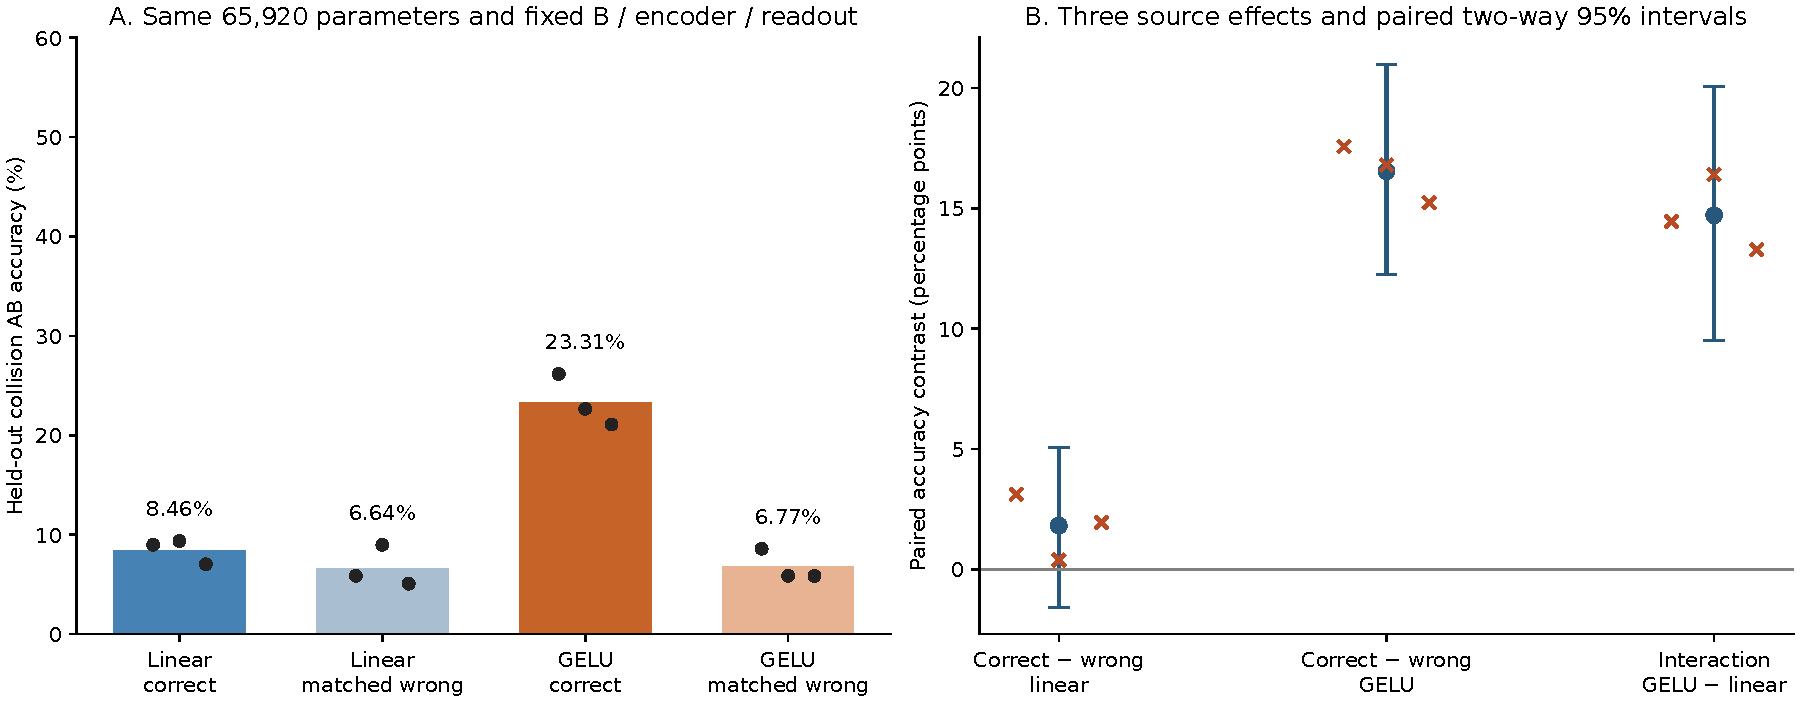
\includegraphics[width=\textwidth]{../results/operator_capacity_confirmation/capacity_confirmation.pdf}
\caption{Parameter-matched four-arm results and paired effects. Dots on accuracy bars and crosses on contrasts show individual source outcomes.}
\end{figure}
\paragraph{Interpretation.}
The registered directional interaction was supported on these three new sources and new test inputs. These results are conditional on a correctly relation-trained frozen encoder and do not demonstrate spontaneous relation discovery. Activation also changes optimization, which cannot be separated from expressivity by this intervention alone. The prior 50.65\% diagnostic used more nonlinear parameters, geometry-only fitting and old sources and tests; it is not a directly matched baseline for the present study. A 50\% information ceiling applies to deterministic encodings of the three gold visible answers, not to full output distributions or hidden states. Exceeding that ceiling does not by itself establish an output-independent mechanism.
\paragraph{Verification.}
17173 independent checks passed, including scalar finite-field action and label reconstruction, orbit exclusion, matched parameter count and exposure schedules, unchanged frozen buffers and shared backbone hashes, and NumPy double-precision replay using scalar erf for GELU. All existing project tests and the new manipulation tests passed. This document is supplied as LaTeX source; a TeX compiler is unavailable in the current environment.
\end{document}
